% this file is called up by thesis.tex
% content in this file will be fed into the main document

%: ----------------------- name of chapter  -------------------------
\chapter{Player Engine Design} % top level followed by section, subsection


%: ----------------------- paths to graphics ------------------------

% change according to folder and file names
\ifpdf
    \graphicspath{{X/figures/PNG/}{X/figures/PDF/}{X/figures/}}
\else
    \graphicspath{{X/figures/EPS/}{X/figures/}}
\fi

\section{Overview}
In chapter 3, I mainly describe the player engine design of the HCMP Player, 
focus will be on how player engine communicate with GUI component, what is the 
function of player engine. In real implementation, the player engine is 
executed in a perfermer thread, and the message queue is like ``pipe'' between 
two programs. The player engine has a timer which will periodically check the
message queue, the period is about 10ms, any user 
input will immediatelly passed to player engine through message queue and 
handled, the latency can be ignored. 

\begin{figure}[H]
\center{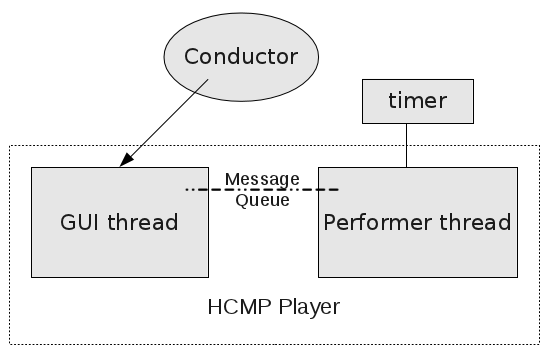
\includegraphics[width=0.55\linewidth]{3/3.png}}
\caption{HCMP GUI Screen Shot}
\label{fig:speciation}
\end{figure}

The player engine has two major functions, the first function is to receive 
command from GUI component, the second function is to schedule and play the
midi note at desire time. So, we can basically divide design of player engine  
into two parts, synchronization and communication. Synchronization refer to
media synchroization, which involv how schedule midi note, how to resposne to
the change of tempo. Communication refer to the way player engine and front-end  
GUI work together.

\section{Media Synchronization}

To accurately schedule the midi note and apply to any tempo chage.  The player 
engine requires two scheduler, one is real-time scheduler. Usually, 
a computation will perform some action needed at the present time,
followed by the scheduling of the next action. The real-time scheduler’s role 
is to keep track of all pending actions and to invoke them at the proper 
time, thus eliminating the need
for Players to busy wait, poll, or otherwise waste computer cycles to 
ensure that their next computation is performed on time. The other 
scheduler is 
a virtual-time player, the virtual-time scheduler is built upon the
real-time player, in most of popular music, we can treat 
synchronization happened at beat level. The purpose of virtual-time
scheduler is to schedule everything at beat level, and the huge 
advantage is that once tempo changed, either due to internal parameter 
of midi file or external signal, there is no need to reschedul 
everything. With virtual-time scheduler, we only need to rearrage
limited number of midi notes.

\subsection{Tempo Prediction}
Assumming most popular music forms has common structure of
beats and measures across all instruments. Thus time is measured in beats. 
The basis for synchronization is a shared notion of the current beat 
and the current tempo. Beats are represented by a floating point number, 
hence they are continuous rather than
integers or messages such as in MIDI clock messages. Also, rather than update the
beat number at frequent intervals, we use a continuous linear mapping from time to
beat. This mapping is conveniently expressed using three parameters (b0, t0, s):
\begin{equation}
b = b_0 + (t - t_0) * s 
\end{equation}

where tempo s is expressed in beats per second, at some time in the past beat b0
occurred at time t0, the current time is t, and the current beat is b. (One could also
solve for b0 when t0 = 0 to eliminate one parameter, but we find this formulation
more convenient)

\begin{figure}[H]
\center{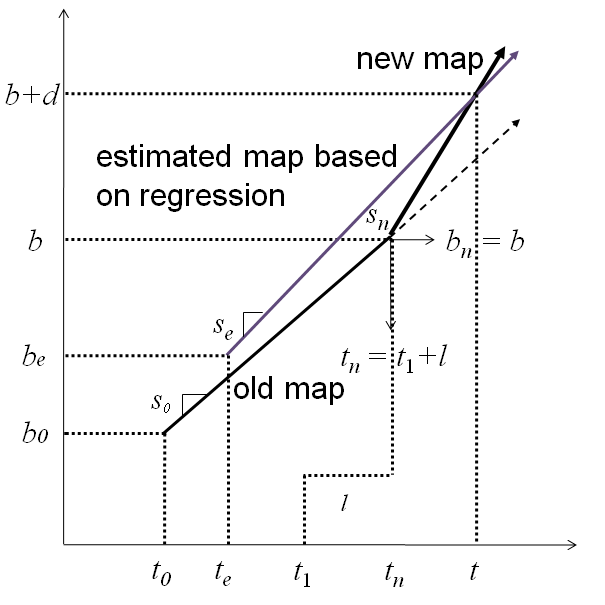
\includegraphics[width=0.5\linewidth]{3/2.png}}
\caption{Midi data display integrated with vitural keyboard}
\label{fig:speciation}
\end{figure}

One advantage of this approach is that it is almost independent of latency.
One can send (t0, b0, s) to another computer or process and the mapping will remain
valid regardless of the transmission latency. When parameters change,
there can be a momentary disagreement in the current time among various
processes, but this should be small given that tempo is normally steady. We will see
below how these slight asynchronies can be smoothed and do not lead to long-term
drift.

Media players schedule computation to affect the output at specific beat
times. For example, an audio player may begin a sample playback at beat 3, or a
MIDI player may send a note-on message at beat 5. The current beat time b in Eq. 1
refers to the beat position of media which are being output currently, e.g. the beat
position corresponding to the current output of a digital-to-analog converter (DAC).
Time-dependent computation of media must of course occur earlier. For example, if
the audio output buffer contains 0.01s of audio, then computation associated with
beat b should be performed 0.01s earlier than b. Thus, given a player-specific latency
l, we need to compute the real time t at which to schedule a computation associated
with beat b. The following formula is easily derived:

\begin{equation}
t = t_0 + (b - b_0) / s - l
\end{equation}

We simply map the beat position b according to (b0, t0, s), and then subtract the
latency l to get the computation time t.

Our current scheduelr use a simple method to predict the beat . 
Basically, a linear regression over recent taps is used to estimate the
mapping from beat to time (i.e. to estimate t0, b0, and s). At this stage, successive
beats are numbered with successive integers, but these start at an arbitrary number.
Once the tempo and beat phase is established, there must be some way to determine
an offset from the arbitrary beat number to the beat number in the score. This might
be determined by a external signal that tells when the system should begin 
to play. In other cases, especially with a foot-pedal interface, 
the system can be constructed to, say,
start on the third beat
Aaudio analysis could be used to automate beat identification
to a large extent, and research investigating combinations of automated 
and manualtechniques has been made and proofed to achieve high reliability 
for live performance. The
important point here is that some mechanism estimates a local mapping between
time and beat position, and this mapping is updated as the performance progresses.

\subsection{Scheduling}

Schedulers in the HCMP Player accept requests to perform specific
computations at specific times in the future. Sometimes, the specified time 
can be a ``virtual'' time in units such as beats that are translated to real 
time according to a
(possibly varying) tempo, as in Eq. 3.2. An important idea is
that all pending events (callbacks) can be sorted according to beat time 
and then one need only worry about the earliest event. If the tempo 
changes, only the time of this
earliest event needs to be recomputed. When event times are
computed according to Eq. 3.2, the earliest pending event can change when tempo
changes. 

\section{Communication}

Figure 3.3 illustrate commuication between GUI and player engine, in this figure,  
the GUI component will be ``front-end'' part of HCMP Plaer, and player engine   
is the ``back-end'' part. In stand-alone mode, the GUI receive request from  
user input by clicking a button, adjustting a slider bar. These events will be  
captured by GUI component, processed and evnentualy passed to player engine. 
In network mode, we could 
treat request from remote server as virtual user request, player engine has no 
idea whether the request is generated by a user's motion or a remote server. Based
on this scenaio, a unified API between GUI component and player engine is defined to
clearly illustrate the responsiblity of each module. Note that the API between 
GUI component and player engine is different from that of network API, the 
former is an internal API between two module, the latter is defined to coordiate
between remote server and multiple instance of HCMP players.

\begin{figure}[H]
\center{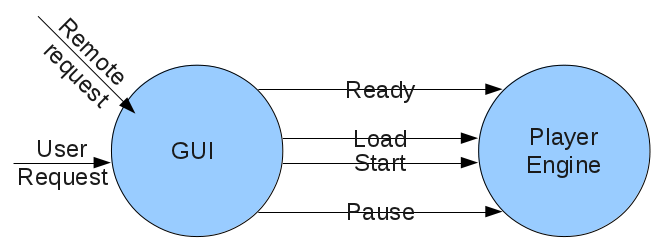
\includegraphics[width=0.7\linewidth]{3/4.png}}
\caption{GUI and Player Engine}
\label{fig:speciation}
\end{figure}

\subsection{Graphic User Interface Thread}

The table 3.2 list the GUI component and its behaviour, in stand-alone 
when user click above button it will send request to player engine.
\begin{table}[htdp]
\centering
\begin{tabular}{|l||*{2}{c|}}\hline
GUI component & Send Request \\ \hline
load button & load\_file \\\hline
play button & play\\\hline
pause button & pause \\\hline
stop button & stop \\\hline
network button & send\_con\_req \\\hline
tempo slider & change\_tempo \\\hline
volume slider & change\_volume \\\hline
\end{tabular}

\caption[GUI component and request]{GUI component and request}
\label{latexin_genes}
\end{table}

\subsection{State Transition Diagram}

Table 3.2 and 3.3 are state transition diagrams for player engine. Column is state, 
Row is method,  each pair in the table means that, given state and method, 
what player engine will transit to.

The player engine only receive control messages from GUI component . 
It immediately process the message upon receiving it. The player engine 
will periodically be invoked by 
a external timer, and process midi request sent from the control thread. 
Processing the request is not a time consuming job so the overall overhead 
of waking up thread will be trivial. 

\begin{table}[htdp]
\centering
\begin{tabular}{|l||*{6}{c|}}\hline
\backslashbox{State}{Method}
&\makebox load & play & pause & stop \\\hline\hline
uninitialize & ready & undefine & undefine & undefine \\\hline
ready & ready & pause & ready & undefine \\\hline
playing & ready & playing & pause & ready \\\hline
pause & ready & playing & pause & ready  \\\hline
network& con\_ready & undefine & con\_suspend& undefine\\\hline 
\end{tabular}

\caption[Player Engine State Transition Diagram]{Player Engine State Transition Diagram}
\label{latexin_genes}
\end{table}

\begin{table}[htdp]
\centering
\begin{tabular}{|l||*{2}{c|}}\hline
\backslashbox{State}{Method}
&\makebox change\_tempo & change\_volume\\\hline\hline
uninitialize &  undefine & undefine \\\hline
ready & undefine & undefine \\\hline
playing & apply\_change & apply\_change \\\hline
pause  & apply\_change & apply\_change \\\hline
network & undefine & undefine \\\hline 
\end{tabular}
\caption[Player Engine State Transition Diagram]{Player Engine State Transition Diagram}
\label{latexin_genes}
\end{table}
\section{Player Engine Programming Interface}
In this section, I list all of the APIs GUI use to communication with player 
the GUI and player will communicate with each other using strings and 
all the parameter is of type string. For example, 
\texttt{"method\_name;argument1;argument2;argument3"}, the argument is 
separated by a \texttt{";"}
character. When passing in the parameter string, the player engine will 
use a function similar to \texttt{split} to store each elment into an
array and invoke according method. These functions maybe different
from the those APIs define in next chapter, but they are quite similar\\
Player control related APIs 
\begin{itemize}
  \item \texttt{load - "load;file\_path"}
  \item \texttt{play - "play;void"}  
  \item \texttt{pause - "pause;void"}
  \item \texttt{stop - "stop;void"}
\end{itemize}
Audio control related APIs
\begin{itemize}
  \item \texttt{change\_volume - "change\_volume;track\_num;velocity"}  
  \item \texttt{change\_tempo - "change\_tempo;tempo\_scale\_coefficient"}  
\end{itemize}
Connection mode related APIs, detail define in following chapter.
\begin{itemize}
  \item \texttt{ini\_connection - "ini\_connection;void"}  
\end{itemize}
